\section{Problem 8}

\subsection{Code}

\begin{lstlisting}
clc; clear all; close all; format long g;
%----- Setup
Tfull = 0.5;     % Time interval of data to load
fs = (40/7)*1e6; % IQ sampling frequency (Hz)
Ts = 1/fs;
N = floor(fs*Tfull/16)*16;
nfft = 2^9;      % Size of FFT used in power spectrum estimation
%----- Load data
fileName = 'dataout_raw_trimmed_158.bin';
fid = fopen(fileName,'r','l');
[yhist,count] = binloadSamples(fid,N,'dual');
yhist = yhist(:,1);
fclose(fid);

%----- Compute power spectrum estimate
[Syy,fVec] = pwelch(yhist,hann(nfft),[],nfft, fs);
plotPSD(Syy, fVec, nfft, fs, -63, -55);

% Convert signal to its baseband representation and compute PSD
fIF = 1610476.187;
[IVec,QVec] = if2iq(yhist, Ts, fIF);
xVec = IVec + j*QVec;
[Syy_IQ, fVec_IQ] = pwelch(xVec,hann(nfft),[],nfft, fs/2);
plotPSD(Syy_IQ, fVec_IQ, nfft, fs, -63, -55);

tau = (Ts*2)*(0:1:N-1)'; % sampling time (in RX time base)

fStep = 10; % Hz
nStep = 1;  % Ts
for TXID = 1:37
    [fDk_hat(TXID), tsk_hat(TXID), C_N0_hat(TXID), detected(TXID)] = 
                    acquireGPS(tau, xVec, Ts*2, 5, fStep, nStep, TXID, 'FFT');
end
\end{lstlisting}

\begin{lstlisting}
%%%%%%%%%%%%%%%%%%%%%%%%%%%%%%%%%%%%%%%%%%%%%%%%%%%%%%%%%%%%%%%%%%%%%%%%%%%%%%%%
function [fdk_hat, tsk_hat, C_N0, isAcquired] = acquireGPS(tau, x, T, nTc,...
                                                fStep, nStep, TXID, method)
% Spreading code replica
Nc = 1023;
Tc = 1e-3/Nc;
code = generatePRN(TXID); 

% generate data for the k-th accumulation 
Ta = nTc*Nc*Tc;
Nk = floor(Ta/T);
tau = tau(1:Nk);
x   = x(1:Nk);

% resample C at TsamplingIQ
code = repmat(code, [nTc 1] );
C = oversampleSpreadingCode(code, T/Tc, 0, Nk, Nc);

epsilon = 50*(nTc/Ta);
fDk_hat = -epsilon:fStep:epsilon;
M = zeros(Nk,length(fDk_hat));
if strcmp(method, 'FFT')
    Cr = fft(C);
    parfor fDk_idx = 1:length(fDk_hat)
        % phase estimate over the accumulation interval
        theta_jk_hat = 0;
        theta_hat = 2*pi*fDk_hat(fDk_idx)*tau + theta_jk_hat;

        x_tilde = x.*exp(-i*theta_hat);
        Xr_tilde = fft(x_tilde);
        Zr = Xr_tilde.*conj(Cr);
        zk = ifft(Zr);
        
        M(:,fDk_idx) = abs(zk).^2;
    end
else
    parfor fDk_idx = 1:length(fDk_hat)
        for n = 1:nStep:Nk            
            % phase estimate over the accumulation interval
            theta_jk_hat = 0;
            theta_hat = 2*pi*fDk_hat(fDk_idx)*tau + theta_jk_hat;
            
            % Align C with the code in the incoming data.
            Cshift = circshift(C,n-1);

            % Calculate Sk and store in a matrix that represents the 2D-grid
            Sk = sum(x.*exp(-i*(theta_hat)).*Cshift);
            M(n, fDk_idx) = abs(Sk)^2;
        end
    end
end

% % DEBUG
% tau_jk = tau(1:Nk)*1e6;
% ii = find(tau_jk<1000);
% figure();
% h = surf(fDk_hat, tau_jk(ii), M(ii,:));
% set(h,'LineStyle','none')
% title('2D grid - S_k')
% xlabel('$\hat{f}_{Dk} [Hz]$','Interpreter','latex')
% ylabel('$\tau_{jk} [us]$','Interpreter','latex')

% Find the maximum Sk in the 2D-grid
[max_Sk, max_idx] = max(M(:));
[n, fDk_idx]=ind2sub(size(M),max_idx);

% Estimates
isAcquired = max_Sk > 1.5e6;
fdk_hat = fDk_hat(fDk_idx); % Hz
tsk_hat = tau(n)*1e6;       % us 

two_sigmaIQ_squared = 61551.7110161536; % mean(M,'all') for satellite 34
%two_sigmaIQ_squared = 568409076.119826; % mean(M,'all') for satellite 34
C_N0 = 10*log10((max_Sk - two_sigmaIQ_squared)/(two_sigmaIQ_squared*Ta));

end
%%%%%%%%%%%%%%%%%%%%%%%%%%%%%%%%%%%%%%%%%%%%%%%%%%%%%%%%%%%%%%%%%%%%%%%%%%%%%%%
\end{lstlisting}


\subsection{Results}

\begin{tabular}{c|c|c|c}
	PRN & Doppler [MHz] & $\tau$ [$\mu s$] & C/N0   \\
	\hline
	1   & $-33.840$     & 410              & $48$   \\
	11  & $-35.910$     & 578              & $48.9$ \\
	14  & $-20.280$     & 35               & $38.8$ \\
	18  & $-34.220$     & 370              & $50$   \\
	31  & $-25.350$     & 804              & $40.9$ \\
\end{tabular}


\begin{figure}[H]
	\centering
	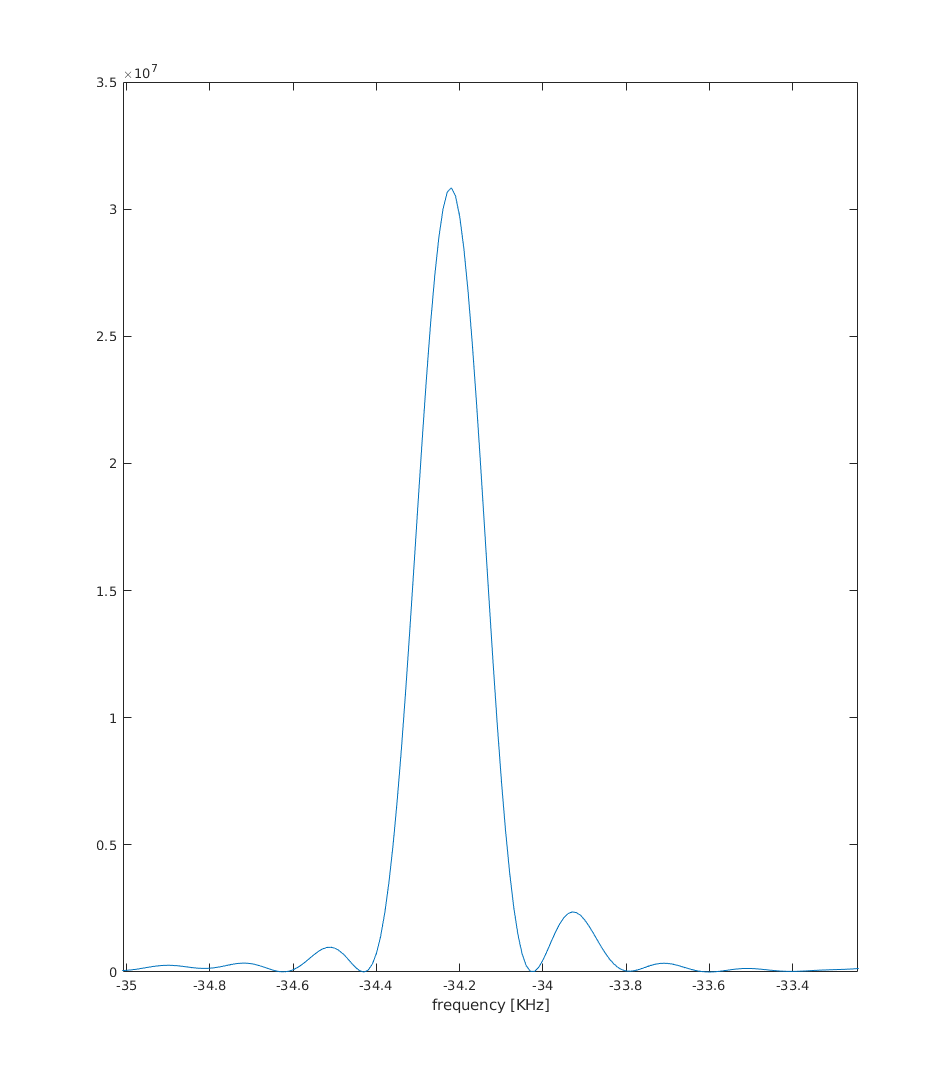
\includegraphics[width=0.9\textwidth]{figs/Sk_freq.png}
	\caption{$|S_k| vs \hat{f}_{D,k}$ for the maximizing $\hat{t}_{s,k}$.}
	\label{fig:sk_freq}
\end{figure}

\begin{figure}[H]
	\centering
	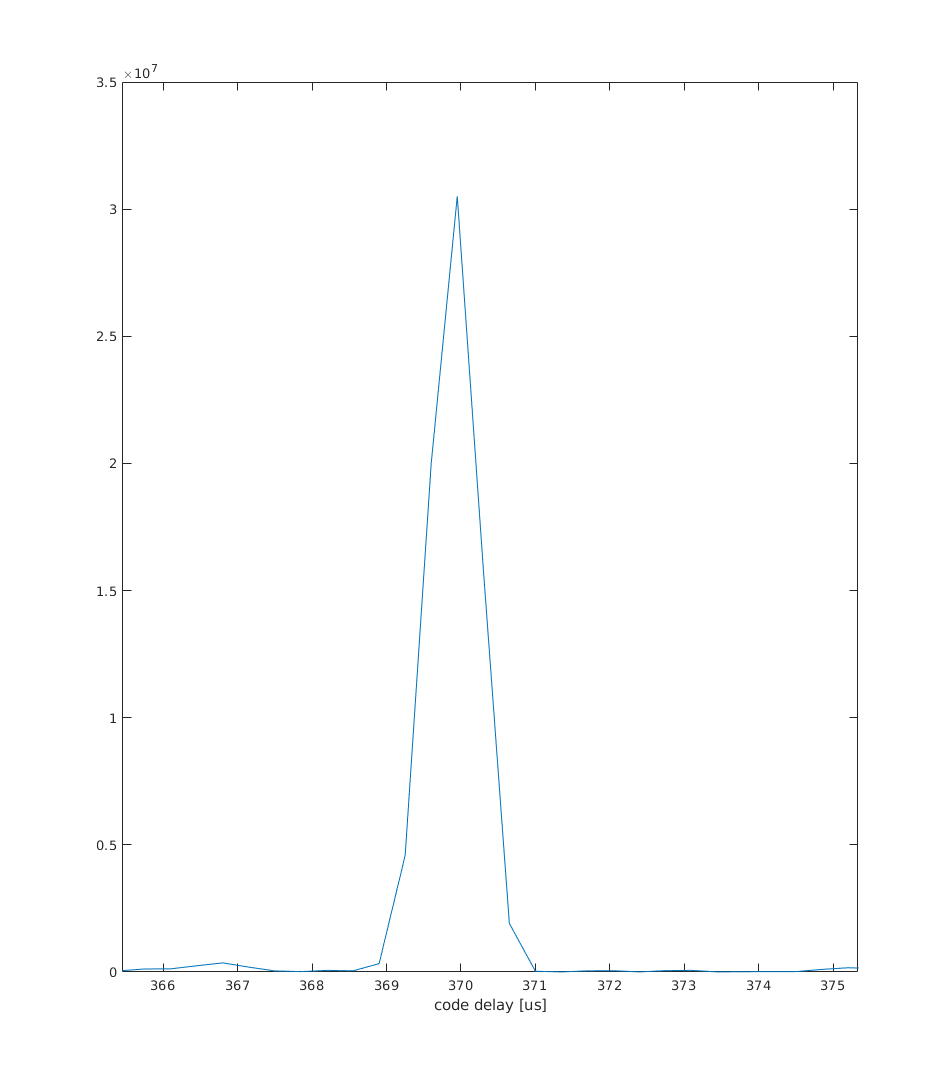
\includegraphics[width=0.9\textwidth]{figs/Sk_tau.png}
	\caption{$|S_k| vs \hat{t}_{s,k}$ for the maximizing $\hat{f}_{D,k}$.}
	\label{fig:sk_tau}
\end{figure}
